% main.tex — Root document
\input{preamble}

\begin{document}

\maketitle

\begin{abstract}
A short description of your research project.
\end{abstract}

\tableofcontents
\newpage

\section{Introduction}

This is the introduction. Replace this with your content.


\section{Methods}

This is the methods section. Describe your approach here.

\section{Results}


\subsection{Linear Model}

Figure~\ref{fig:linear-model} shows the results.

\begin{figure}[H]
  \centering
  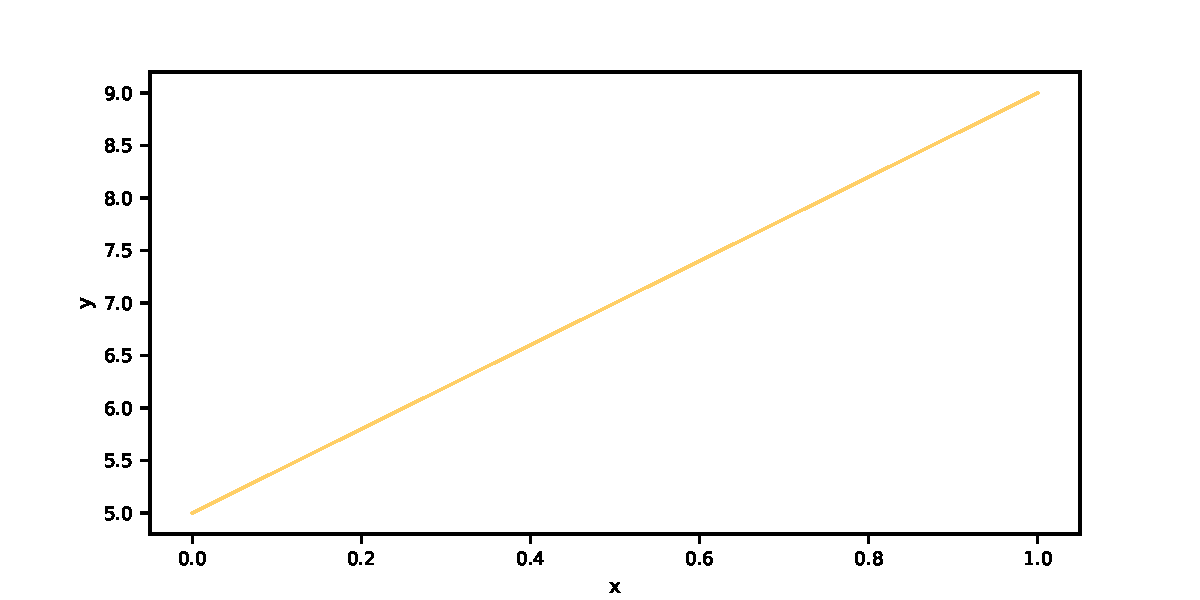
\includegraphics[width=0.7\textwidth]{figures/plot.pdf}
  \caption{The linear model.}
  \label{fig:linear-model}
\end{figure}

\section{Conclusion}

Summary of findings and future work.

\appendix
\section{Input Assumptions}

Figure~\ref{fig:datacenter_demand} shows the assumptions for
electricity demand from datacenters. The load profile is assumed
constant, and a corresponding demand response potential is assumed for
configurations with flexible datacenter demand. This is based on TYNDP
2024 \cite{entso-eTYNDP2024Scenarios2025}, and no assumptions are made
in order to extrapolate this database to non-EU member states such as
Norway and United Kingdom. Hence, demand for datacentres is zero in
these countries.

\begin{figure}[H]
  \centering
  
\includegraphics[width=0.7\textwidth]{figures/datacenter_electricity_consumption.pdf}
  \caption{Assumptions for annual datacenter electricity demands, based on TYNDP 2024.}
  \label{fig:datacenter_demand}
\end{figure}

% Bibliography
\bibliography{bibliography}
\bibliographystyle{apalike}

\end{document}
